\documentclass[11pt,a4paper]{article}

%%%%%%%%%%%%%%%%%%%%%%%%%%%%%%%%%%
% Encoding and language
\usepackage[utf8]{inputenc}
\usepackage[T1]{fontenc}
\usepackage[english]{babel}
\selectlanguage{English}

%%%%%%%%%%%%%%%%%%%%%%%%%%%%%%%%%%
% General packages
\usepackage{verbatim}
\usepackage[all]{xy}
\usepackage{float}
\usepackage{amsmath}
\usepackage{array}
\usepackage{listings}
\usepackage{xcolor}
\usepackage{setspace}
\usepackage{booktabs}
\usepackage{graphicx}
\usepackage{url}
\usepackage{lmodern}
\interfootnotelinepenalty=10000

%%%%%%%%%%%%%%%%%%%%%%%%%%%%%%%%%%
% Page layout
\usepackage{geometry}
\geometry{margin=2.5cm}

%%%%%%%%%%%%%%%%%%%%%%%%%%%%%%%%%%
% Hyperlinks
\usepackage[
    colorlinks=true,
    urlcolor=blue!50!black,
    linkcolor=black,
    citecolor=black
]{hyperref}

%%%%%%%%%%%%%%%%%%%%%%%%%%%%%%%%%%
% Bibliography
\usepackage[round]{natbib}

%%%%%%%%%%%%%%%%%%%%%%%%%%%%%%%%%%
% Fancy headers (ALL pages incl. title page)
\usepackage{fancyhdr}
\pagestyle{fancy}

\fancyhf{} % clear header/footer

\fancyhead[L]{zpn710, fps618, kvb125, xnc401 - everyone contributed equally}
\fancyhead[R]{February 2026}
\fancyfoot[C]{\thepage}

\renewcommand{\headrulewidth}{0.4pt}
\renewcommand{\footrulewidth}{0pt}

% IMPORTANT: make 'plain' style match 'fancy'
\fancypagestyle{plain}{
    \fancyhf{}
    \fancyhead[L]{zpn710, fps618, kvb125, xnc401 - everyone contributed equally}
    \fancyhead[R]{February 2026}
    \fancyfoot[C]{\thepage}
    \renewcommand{\headrulewidth}{0.4pt}
}

%%%%%%%%%%%%%%%%%%%%%%%%%%%%%%%%%%
% Listings styles
\lstdefinestyle{CStyle}{
    language=C,
    basicstyle=\small\ttfamily,
    keywordstyle=\color{blue},
    commentstyle=\color{green!40!black},
    stringstyle=\color{orange},
    numbers=left,
    numberstyle=\tiny,
    stepnumber=1,
    numbersep=5pt,
    backgroundcolor=\color{gray!5},
    frame=single,
    rulecolor=\color{black!30},
    captionpos=b,
    breaklines=true,
    breakatwhitespace=true,
    tabsize=4,
    showspaces=false,
    showstringspaces=false,
}

\definecolor{bluekeywords}{rgb}{0.13,0.13,1}
\definecolor{greencomments}{rgb}{0,0.5,0}
\definecolor{turqusnumbers}{rgb}{0.17,0.57,0.69}
\definecolor{redstrings}{rgb}{0.5,0,0}

\lstdefinelanguage{FSharp}{
    morekeywords={let,new,match,with,rec,open,module,namespace,type,of,member,and,for,in,do,begin,end,fun,function,try,mutable,if,then,else},
    keywordstyle=\color{bluekeywords},
    sensitive=false,
    morecomment=[l][\color{greencomments}]{///},
    morecomment=[l][\color{greencomments}]{//},
    morecomment=[s][\color{greencomments}]{{(*}{*)}},
    morestring=[b]",
    stringstyle=\color{redstrings}
}

%%%%%%%%%%%%%%%%%%%%%%%%%%%%%%%%%%
% Matrix spacing fix
\makeatletter
\renewcommand*\env@matrix[1][*\c@MaxMatrixCols c]{%
  \hskip -\arraycolsep
  \let\@ifnextchar\new@ifnextchar
  \array{#1}}
\makeatother

%%%%%%%%%%%%%%%%%%%%%%%%%%%%%%%%%%
% Graphics paths
\graphicspath{{figures/}{anotherFigureDirectory/}}

%%%%%%%%%%%%%%%%%%%%%%%%%%%%%%%%%%
% Title (no author/date under title)
\title{\LARGE \textbf{Handin 2 Numerical Optimization} \\[1ex]}
\date{}

\makeatletter
\def\@maketitle{%
  \newpage
  \null
  \vskip 1em % ← space above title (adjust if you want)
  \begin{center}%
    {\LARGE \bfseries \@title \par}%
    \vskip 0.5em % ← space below title (THIS controls the gap)
  \end{center}%
}
\makeatother

%%%%%%%%%%%%%%%%%%%%%%%%%%%%%%%%%%
\begin{document}

\maketitle

\section{Introduction}

This report presents the analysis of function \(f_5\) in two dimensions, deriving the Newton step direction and demonstrating Q-linear convergence. We implement Newton's algorithm with backtracking line-search and benchmark its performance against steepest descent and BFGS algorithms. The results from the theoretical predictions align with the empirical outcomes.

\section{Theoretical Assignment}

Given \(d=2\) we have,
\[
f_5(x)=\sum_{i=1}^2 |x_i|^{a_i},\qquad 
a=2\cdot \mathrm{linspace}(1,2,2)=[2,4]
\]
and therefore
\[
f_5(x_1,x_2)=|x_1|^2+|x_2|^4,\qquad x^*=(0,0)^T
\]

\paragraph{Gradient and Hessian (for \(x_2\neq 0\)).}
Using \(\frac{d}{dx}|x|^a=a|x|^{a-1}\operatorname{sign}(x)\) for \(a>1\),
\[
\nabla f_5(x)=
\begin{pmatrix}
2\,\operatorname{sign}(x_1)|x_1|^{1}\\[2pt]
4\,\operatorname{sign}(x_2)|x_2|^{3}
\end{pmatrix}
=
\begin{pmatrix}
2x_1\\
4\,\operatorname{sign}(x_2)|x_2|^{3}
\end{pmatrix}
\]
For the Hessian (we note that \(|x_2|^4=x_2^4\) for \(x_2\neq 0\)),
\[
H_{f_5}(x)=
\begin{pmatrix}
2 & 0\\
0 & 12x_2^2
\end{pmatrix}
=
\begin{pmatrix}
2 & 0\\
0 & 12|x_2|^2
\end{pmatrix}
\]

\paragraph{Newton step}
\[
p_k=-H_{f_5}(x_k)^{-1}\nabla f_5(x_k)
\]
Since \(H_{f_5}\) is diagonal,
\[
p_k=
-\begin{pmatrix}
\frac12 & 0\\
0 & \frac{1}{12|x_{k,2}|^2}
\end{pmatrix}
\begin{pmatrix}
2x_{k,1}\\
4\,\operatorname{sign}(x_{k,2})|x_{k,2}|^3
\end{pmatrix}
=
\begin{pmatrix}
-x_{k,1}\\[2pt]
-\frac{1}{3}\operatorname{sign}(x_{k,2})|x_{k,2}|
\end{pmatrix}
=
\begin{pmatrix}
-x_{k,1}\\
-\frac{1}{3}x_{k,2}
\end{pmatrix}
\]

\paragraph{Iteration with \(\alpha_k=1\)}
\[
x_{k+1}=x_k+p_k=
\begin{pmatrix}
0\\
\frac{2}{3}x_{k,2}
\end{pmatrix}
\]
and therefore
\[
\|x_{k+1}-x^*\|=\frac{2}{3}\|x_k-x^*\|,
\]
so Newton’s method is Q-linear with rate
\[
r=\frac{2}{3},
\]
and not Q-superlinear since
\[
\lim_{k\to\infty}\frac{\|x_{k+1}-x^*\|}{\|x_k-x^*\|}=\frac{2}{3}\neq 0
\]

\paragraph{Generalization to \(d>2\).}
We did not have space to show this generalization. A rough sketch is as follows: since the function is a sum of non-mixed terms, the Hessian is diagonal. Hence Newton acts coordinatewise, and each component is multiplied by a fixed scalar independent of k. We believe that this would mean that the contraction rate would be constant as before.


\section{Programming Assignment}

\subsection{Testing protocol and Results}
For each test function, multiple random initial points are sampled, and all algorithms are initialized from the same points. We sampled 100 initial points from a multivariate Gaussian $\text{N}(x^*,100 \cdot \text{I})$ centered at each function's optimum. Each algorithm is run until convergence or until a maximum number of iterations is reached. Convergence requires the norm of the gradient to fall below a fixed tolerance~$\varepsilon = 10^{-8}$.

For each algorithm, we have plotted the median convergence trajectory over multiple random initializations is shown, together with a shaded region representing the range 50th to 75th percentile. This is shown in Figure ~\ref{fig:newtonsplot}. The 99th percentile is additionally included to capture rare but extreme convergence behavior. The y-axis is cut to the tolerance $\varepsilon=10^{-8}$. We also added a new plot that tracked the convergence rate for the algorithm starting at 2 points (1,1) and (10,10).

\begin{figure}[H]
    \centering
    \includegraphics[width=1\textwidth]{newtonsplot.png}
    \caption{
    Median convergence trajectories with 75th percentile band and 99th percentile.
    }
    \label{fig:newtonsplot}
\end{figure}

\begin{figure}[H]
    \centering
    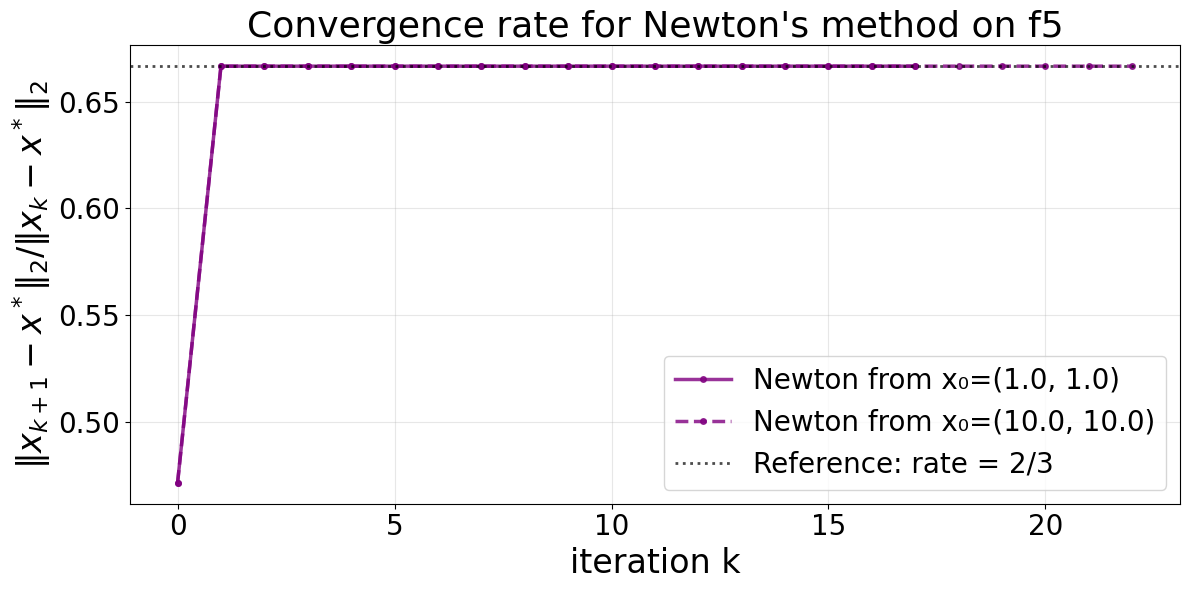
\includegraphics[width=0.8\textwidth]{convergence_rate.png}
    \caption{
    Convergence rate for Newtons method where $\alpha_k = 1$
    }
    \label{fig:convergence}
\end{figure}


\subsection{Do the theoretical and empirical results for $f_5$ correspond?} 
As shown in figure \ref{fig:convergence} the convergence rate of $2/3$ matches the rate calculated in the theoretical section. We ran tests to find out why it does not match for the first step, but we did not find any satisfactory answers. However, one could argue that the convergence rate in the first step is insignificant when taking the number of total steps into account. 

\subsection{Is your implementation of the algorithm correct?} 
Yes, we strongly believe that our implementation of the algorithm is correct. This is shown by the exact matching convergence rate and core structure built around the pseudo-code of algorithm 4 in the theoretical course material.

\subsection{Do the algorithms perform well?}
As shown in figure \ref{fig:newtonsplot} we found that the steepest descent algorithm is slow and for $f_2$ it does not reach the $\varepsilon$ threshold. Our newly implemented Newtons method works the best on all 5 functions. We believe that this is because newtons method uses more information as it uses the hessian and not just the gradient.

\section{Conclusion}

Our findings demonstrates both theoretically and empirically that Newton's method achieves Q-linear convergence with rate $r=2/3$ for function $f_5$ in two dimensions. Newton's method consistently outperforms steepest descent and BFGS across all test functions. These results confirm the advantage of incorporating second-order derivative information in the optimization algorithms.

\end{document}
